% !TeX spellcheck = fa
\documentclass[a4paper,12pt]{report}

\usepackage{color}
\usepackage{fourier}
\usepackage{amsmath}
\usepackage{dirtree}
\usepackage{caption}
\usepackage{verbatim}
\usepackage{fancyhdr}
\usepackage{graphicx}
\usepackage{outlines}
\usepackage{enumitem}
\usepackage{fancyvrb}
\usepackage{listings}
\usepackage{makecell}
\usepackage{tabularx} % for custom width table
\usepackage{subcaption}
\usepackage{indentfirst}
\usepackage{lstautogobble}
\usepackage[table]{xcolor}
%% \usepackage[perpage]{footmisc}
\usepackage[breakable]{tcolorbox}
\usepackage[Bjornstrup]{fncychap}%Options: Sonny, Lenny, Glenn, Conny, Rejne, Bjarne, Bjornstrup
\usepackage[colorlinks,linkcolor=blue,citecolor=red,urlcolor=blue]{hyperref}
\tcbuselibrary{breakable, skins}
\usepackage[logo=on,fontsize={12,18}]{xepersian}

% -------------- tcolorbox -------------
\tcbset{
	enhanced,
	colback=cyan!5!white,
	boxrule=0.1pt,
	colframe=cyan!75!black,
	fonttitle=\bfseries,
	width=0.9\linewidth
}
% -------------- xepersian -------------
%% \settextfont{Microsoft Sans Serif}
\settextfont{XB Yas}
\setlatintextfont{XB Yas}

\defpersianfont\Title[Scale=1.1]{XB Titre}
\deflatinfont\InTheNameOfGod[Scale=16]{Far.Symbol8}

% --------------   xcolor  -------------
\definecolor{ao}{rgb}			{0.00, 0.50, 0.00}
\definecolor{codeGreen}{rgb}	{0.00, 0.50, 0.50}
\definecolor{lavendergray}{rgb}	{0.87, 0.86, 0.92}
\definecolor{mint}{rgb}			{0.24, 0.71, 0.54}
\definecolor{aliceblue}{rgb}	{0.94, 0.97, 1.00}
\definecolor{commentGreen}{rgb}	{0.13, 0.65, 0.47}
\definecolor{steelBlue}{rgb}	{0.00, 0.00, 0.50}
\definecolor{stringGreen}{rgb}	{0.00, 0.50, 0.00}
\definecolor{rowBlue}{rgb}		{0.48, 0.81, 0.87}

% --------------  fancyhdr -------------
\pagestyle{fancy}

\cfoot{\thepage}
\rhead{\thepage }
\renewcommand{\headrulewidth}{0.4pt}

%% new commonds.
\newcommand{\lrm}[1]{\textcolor{steelBlue}{\lr{\texttt{#1}}}}

%% tabular borders color 
\arrayrulecolor{gray}

\begin{document}
	\lstset{
		frame=tb,
		basicstyle	=\color{steelBlue}\linespread{0.8}\ttfamily,
		columns=fullflexible,
		keepspaces	=false,
		tabsize		=3,
		autogobble,
		breaklines	=true,
		breakatwhitespace=true,
		stringstyle	=\color{stringGreen},
		commentstyle=\color{gray},
		keywordstyle=\color{purple},
		language	=c++,
		aboveskip	=3mm,
		belowskip	=3mm,
		showstringspaces=false,
		columns		=flexible,
		captionpos	=b,
		numbers		=left,
		numbersep	=5pt,
		numberstyle	=	\color{gray}\linespread{0.8}\ttfamily,
		postbreak	=	\mbox{\textcolor{blue}{$\hookrightarrow$}\space}
	}
	
	\renewcommand{\bibname}{مراجع}
	\thispagestyle{empty}
	
	\begin{center}
		{
			\qquad\InTheNameOfGod 8
		}
	\end{center}
	\title{
		\Title
		سیستم مدیریت کلینیک
	}
	\author{
		\Title
		وَحید صَدرْنیاٰ، سیّد مرتضیٰ رضوی\\
	}
	\date{
		\Title
		یکشنبه، ۶ اردیبهشت ۱۳۹۹
	}
	
	\pagenumbering{roman}
	\setcounter{page}{0}
	\maketitle
	\tableofcontents
	\listoffigures

	\chapter{
	مستندات طراحی}
	\pagenumbering{arabic}
	\section*{
		مقدمه}
	\label{chap13}
	
	درمانگاه یا کلینیک 
	\LTRfootnote{\lr{Clinic /ˈklɪnɪk/}}
	ساختمان یا بخشی در بیمارستان یا مرکز بهداشتی - درمانی که به درمان بیماران یا مراقبت پزشکی از بیماران سرپایی اختصاص دارد. معمولاً، درمانگاه موسسه‌ای مستقل است که به درمان بیماران می‌پردازد ولی برخلاف بیمارستان، بیماران را بستری نمی کند. درمانگاه می‌تواند عمومی یا تخصصی (مانند درمانگاه پوست و مو یا درمانگاه دندانپزشکی) باشد. برخلاف ساختمان پزشکان، درمانگاه مؤسسه واحدی است لذا می‌تواند با سازمان‌های بیمه گر و ادارات قرارداد (جهت پذیرش بیماران) ببندد.
	
	با توجه به پیشرفت فناوری اطلاعات و نیاز به بروزرسانی سیستم سلامت کشور به این نتیجه رسیدیم که بخش کوچکی از نیازهای فناوری اطلاعات بخش سلامت کشور را تامین کنیم و در این جهت به  پیاده سازی سیستم مدیریت درمانگاه پرداختیم، که نیازمندی‌های صاحب سیستم بطور مفصل در ذیل شرح داده شده‌اند.
	
	\section{نیازمندی‌ها}\label{sec1:chap1}
	\begin{enumerate}[nosep]\label{enum1:sec1:chap1}
		\item 
		مدیرت مالی : این سیستم باید قابلیت مدیریت امور مالی کلینیک را داشته باشد.				
		\item 
		پشتیبانی از نوبت‌دهی آنلاین: در صورت نیاز نوبت دهی آنلاین از طریق وب‌سایت و به صورت غیر حضوری امکان پذیر است.
		\item 
		 اطلاع رسانی: در صورت نیاز به اطلاع رسانی از طریق پیامک به بیمار اطلاع رسانی  می‌شود.
		\item 
		 گزارشات بیمار: در صورت نیاز، بیمار بتواند پیشینه مراجعه خود به درمانگاه را دریافت کند.		 
		\item 
		حضور غیاب کارکنان: امکان حضور و غیاب کارکنان کلینیک، از جمله: دکتر، منشی و... فراهم باشد.
		\item 
		اطلاع رسانی از طریق وب‌سایت: امکان اطلاع رسانی زمان حضور دکتر در درمانگاه از طریق وب‌سایت وجود داشته باشد.
		
		\item 
		گزارش گیری صحت بیمه: درصورت مراجعه بیمار، بیمه آن به صورت الکترونیک چک شود.
		
	\end{enumerate}
	\section{تیم طراحی}\label{sec2:chap1}
	طراحی این نرم‌افزار شامل تیمی متشکل از:
	\begin{itemize}[nosep]\label{item1:sec2:chap1}
		\item 
		تحلیل‌گر و طراحی سیستم.
		\item 
		برنامه نویس مسلط به
		\lr{C Sharp}
		\item 
		طراح
		\lr{back end} و \lr{front end}
		
	\end{itemize}
	این نرم‌افزار تحت ویندوز می‌باشد و بخش نوبت‌دهی آنلاین و اطلاع رسانی از طریق وب‌سایت توسط سیستم مدیریت محتوا، مدیریت می‌شود.

	\section{تحلیل ریسک}\label{sec3:chap1}
	\subsection{پیاده سازی سیستم}\label{subsec1:sec3:chap1}
	با توجه به کوچک بودن گروه توسعه دهنده برای جلوگیری از ایجاد مشکل در فرایند توسعه و تولید نرم‌افزار از یک برنامه‌نویس و تحلیل‌گر پایگاه‌داده و سیستم، دعوت به همکاری شده تا در صورت مشکل برای افراد تیم پروژه با تأخیر جبران ناپذیر مواجه نشود.
	
	با توجه به توسعه فناوری اطلاعات و بالا رفتن سطح دانش عمومی فناوری اطلاعات در بخش پزشکی، ابراز علاقه مراکز بهداشت درمان به خودکار سازی فرایندها پیش بینی می‌شود که این سیستم بخش بزرگی از نیازمندی‌های درمانگاه‌ها را تامین کرده و بتواند بخش قابل توجهی از سهم بازار را از آن خود کند.
	
	\subsection{استقرار در محیط}\label{subsec2:sec3:chap1}
	\begin{enumerate}[nosep]\label{enum1:subsec2:sec3:chap1}
		\item
			استفاده از چند برنامه‌نویس برای هر بخش و 
			\lr{pair programming}.
		\item
			استفاده از سرویس پشتیبان برای چک کردن صحت بیمه، درصورت قطعی یا از درسترس خارج شدن سرویس جاری.
		\item
			استفاده از سرور‌های داخلی در صورت قطع کلی اینترنت.
		\item
			استفاده از سرور پشتیبان محلی برای حفاظت از اطلاعات.
	\end{enumerate}

		
	\section{تخمین هزینه}\label{sec4:chap1}
	\begin{enumerate}[nosep]\label{enum1:sec4:chap1}
		\item 
		$2$ میلیون هزینه برای استخدام برنامه نویس و طراح پایگاه داده.
		\item 
		$3$ میلیون استخدام طراح رابط کاربری‌.
		\item 
		$1.5$ میلیون هزینه برنامه نویس رابط کاربری.
		\item
		$3$ میلیون هزینه برنامه‌نویس 
		\lr{C Sharp}
		\item 
		$1$ میلیون هزینه سالانه سرور.
		\item
		$5$ میلیون هزینه سرور محلی.
	\end{enumerate}

	\pagebreak
	\section{
		داستان‌های کاربر (سناریو کارت‌ها)		
	}\label{sec5:chap1}
	{
		\footnotesize
		\danger
		نکته: این بخش در جهت بهبود نیاز‌مندی‌های سیستم به اسناد اضافه شده‌است.
	}
	\begin{table}[h]
		\centering
		\begin{tabularx}{\textwidth}{| X | X | X |}
			\hline
			
			\rowcolor{rowBlue}
			\multicolumn{1}{|l|}{\lr{\textbf{Title:}}}
			 & \multicolumn{1}{|l|}{\lr{\textbf{Priority:}}}
			 & \multicolumn{1}{|l|}{\lr{\textbf{Estimate:}}}\\
			\rowcolor{rowBlue}
			مدیریت مالی& 1 & 1 ماه\\
			\hline
			\multicolumn{3}{|l|}{\lr{User Story:}} \\
			\multicolumn{3}{|p{0cm}|}{\makecell[r]{
			به عنوان مدیرت مالی\\
			درخواست ایجاد قابلیت مدیریت امور مالی درمانگاه را برای بهبود عملکرد حسابرسی دارم.
				}} \\
			\hline
			\multicolumn{3}{|l|}{\lr{User Story:}} \\
			\multicolumn{3}{|p{0cm}|}{\makecell[r]{
			1- بهبود عملکرد حسابرسی و حسابداری.\\
			2- سرعت بخشیدن به انجام امور مالی.\\
			3- انجام محاسبات سنگین امور مالی.
				}} \\
			\hline
		\end{tabularx}
		\caption{
		مدیریت مالی}		
		\label{table1:sec5:chap1}
	\end{table}

	\begin{table}[h]
		\centering
		\begin{tabularx}{\textwidth}{| X | X | X |}
			\hline
			
			\rowcolor{rowBlue}
			\multicolumn{1}{|l|}{\lr{\textbf{Title:}}}
			& \multicolumn{1}{|l|}{\lr{\textbf{Priority:}}}
			& \multicolumn{1}{|l|}{\lr{\textbf{Estimate:}}}\\
			\rowcolor{rowBlue}
			حضور غیاب & 1 & 4 هفته\\
			\hline
			\multicolumn{3}{|l|}{\lr{User Story:}} \\
			\multicolumn{3}{|p{0cm}|}{\makecell[r]{	
			به عنوان بخش نگهبانی درمانگاه\\
			درخواست ایجاد حضور غیاب کارکنان به وسیله اثر انگشت و شناسایی آنها  توسط سیستم 
			}} \\
			\hline
			\multicolumn{3}{|l|}{\lr{User Story:}} \\
			\multicolumn{3}{|p{0cm}|}{\makecell[r]{
			1- دقت بالاتر در حضور غیاب.\\
			2- ثبت زمان دقیق ورود و خروج کارکنان.\\
			}} \\
			\hline
		\end{tabularx}	
		\caption{
			حضور غیاب}		
		\label{table2:sec5:chap1}	
	\end{table}

	\pagebreak
	
	\begin{table}[h]
		\centering
		\begin{tabularx}{\textwidth}{| X | X | X |}
			\hline
			
			\rowcolor{rowBlue}
			\multicolumn{1}{|l|}{\lr{\textbf{Title:}}}
			& \multicolumn{1}{|l|}{\lr{\textbf{Priority:}}}
			& \multicolumn{1}{|l|}{\lr{\textbf{Estimate:}}}\\
			\rowcolor{rowBlue}
			ثبت اطلاعات & 1 & 3 هفته\\
			\hline
			\multicolumn{3}{|l|}{\lr{User Story:}} \\
			\multicolumn{3}{|p{0cm}|}{\makecell[r]{
			به عنوان دکتر\\
			درخواست ایجاد یک فرم ثبت اطلاعات بیمار
			}} \\
			\hline
			\multicolumn{3}{|l|}{\lr{User Story:}} \\
			\multicolumn{3}{|p{0cm}|}{\makecell[r]{
			1- بازیابی و مرور راحت‌تر پرونده‌های بیماران.\\
			2- سهولت در امر ارزیابی بیمار در طول زمان.\\
			3- ایجاد یک پایگاه داده داده جامع از اطلاعات بیماران به جهت استخراج اطلاعات آماری.
			}} \\
			\hline
		\end{tabularx}		
		\caption{
			ثبت اطلاعات بیماران}		
		\label{table4:sec5:chap1}
	\end{table}

	\begin{table}[h]
		\centering
		\begin{tabularx}{\textwidth}{| X | X | X |}
			\hline
			\rowcolor{rowBlue}
			\multicolumn{1}{|l|}{\lr{\textbf{Title:}}}		&
			\multicolumn{1}{|l|}{\lr{\textbf{Priority:}}}	&
			\multicolumn{1}{|l|}{\lr{\textbf{Estimate:}}}\\
			
			\rowcolor{rowBlue}
			پذیرش & 1 & 3 هفته\\
			\hline
			\multicolumn{3}{|l|}{\lr{User Story:}} \\
			\multicolumn{3}{|p{0cm}|}{\makecell[r]{
			به عنوان پذیرش 
			درخواست، ارائه پشتیبانی از نوبت دهی آنلاین و نوبت دهی الکترونیک 
			}} \\
			\hline
			\multicolumn{3}{|l|}{\lr{User Story:}} \\
			\multicolumn{3}{|p{0cm}|}{\makecell[r]{
			1- سریع نوبت دهی بیماران.\\
			2- سهولت در امر نوبت گیری.\\
			3- نوبت دهی بدون  نیاز به مراجعه بیمار.\\
			}} \\
			\hline
		\end{tabularx}	
		\caption{
			نوبت دهی آنلاین}		
		\label{table5:sec5:chap1}	
	\end{table}

\pagebreak

	\begin{table}[h]
		\centering
		\begin{tabularx}{\textwidth}{| X | X | X |}
			\hline
			
			\rowcolor{rowBlue}
			\multicolumn{1}{|l|}{\lr{\textbf{Title:}}}
			& \multicolumn{1}{|l|}{\lr{\textbf{Priority:}}}
			& \multicolumn{1}{|l|}{\lr{\textbf{Estimate:}}}\\
			\rowcolor{rowBlue}
			پذیرش بخش 2 & 2 & 3 هفته\\
			\hline
			\multicolumn{3}{|l|}{\lr{User Story:}} \\
			\multicolumn{3}{|p{0cm}|}{\makecell[r]{
			به عنوان پذیرش \\
			درخواست، گزارش گیری صحت بیمه بیماران
			}} \\
			\hline
			\multicolumn{3}{|l|}{\lr{User Story:}} \\
			\multicolumn{3}{|p{0cm}|}{\makecell[r]{
			1- دقت در پذیرش بیماران با بیمه معتبر.\\
			}} \\
			\hline
		\end{tabularx}	
		\caption{
			گزارش گیری صحت بیمه}		
		\label{table6:sec5:chap1}	
	\end{table}

	\begin{table}[h]
		\centering
		\begin{tabularx}{\textwidth}{| X | X | X |}
			\hline
			
			\rowcolor{rowBlue}
			\multicolumn{1}{|l|}{\lr{\textbf{Title:}}}
			& \multicolumn{1}{|l|}{\lr{\textbf{Priority:}}}
			& \multicolumn{1}{|l|}{\lr{\textbf{Estimate:}}}\\
			\rowcolor{rowBlue}
			پذیرش بخش 3& 2 & 3 هفته\\
			\hline
			\multicolumn{3}{|l|}{\lr{User Story:}} \\
			\multicolumn{3}{|p{0cm}|}{\makecell[r]{
			به عنوان بخش پذیرش\\
			درخواست تحویل گزارشات بیمار در صورت درخواست بیمار
			}} \\
			\hline
			\multicolumn{3}{|l|}{\lr{User Story:}} \\
			\multicolumn{3}{|p{0cm}|}{\makecell[r]{
			1- سهولت در انجام تحویل گزارشات بیمار.\\
			}} \\
			\hline
		\end{tabularx}	
		\caption{
			ارائه گزارشات به بیمار}		
		\label{table7:sec5:chap1}	
	\end{table}

\pagebreak

	\begin{table}[h]
		\centering
		\begin{tabularx}{\textwidth}{| X | X | X |}
			\hline
			
			\rowcolor{rowBlue}
			\multicolumn{1}{|l|}{\lr{\textbf{Title:}}}
			& \multicolumn{1}{|l|}{\lr{\textbf{Priority:}}}
			& \multicolumn{1}{|l|}{\lr{\textbf{Estimate:}}}\\
			\rowcolor{rowBlue}
			پذیرش بخش 4& 2 & 5 هفته\\
			\hline
			\multicolumn{3}{|l|}{\lr{User Story:}} \\
			\multicolumn{3}{|p{0cm}|}{\makecell[r]{
			به عنوان بخش پذیرش\\
			اطلاع رسانی به بیماران از طریق پیامک و سایت
			}} \\
			\hline
			\multicolumn{3}{|l|}{\lr{User Story:}} \\
			\multicolumn{3}{|p{0cm}|}{\makecell[r]{
			1- یاد آوری بیمار جهت زمان ویزیت.\\
			2 -صرفه جویی در زمان پیرو تاخیر بیمار و اتفاقات پیش‌بینی نشده.\\
			}} \\
			\hline
		\end{tabularx}	
		\caption{
			ایجاد بخش اطلاع رسانی}		
		\label{table8:sec5:chap1}	
	\end{table}

	\pagebreak
	
	\section{تخمین زمان}\label{sec6:chap1}
	\begin{figure}[!h]
		\label{fig1:sec5:chap1}
		\begin{flushleft}	
			\qquad\qquad		
			\begin{subfigure}[t]{0.5\textwidth}
				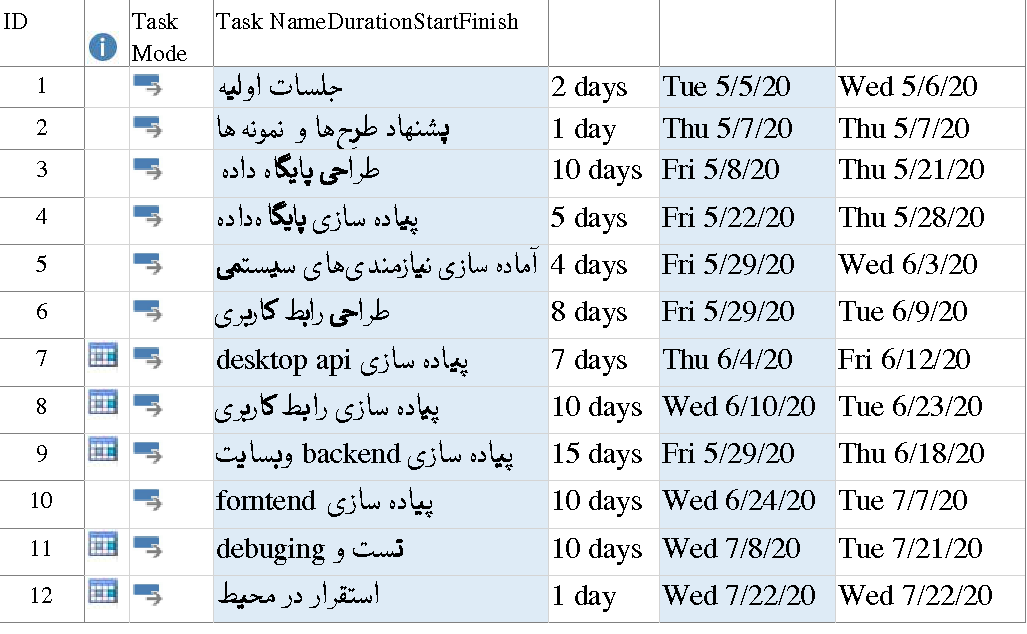
\includegraphics[width=\textwidth]{diagrams/gantChart_timeTable.pdf}
				\caption{جدول زمانی}
				\label{subfig2:fig1:sec5:chap1}
			\end{subfigure}\\
			\begin{subfigure}[t]{\textwidth}
				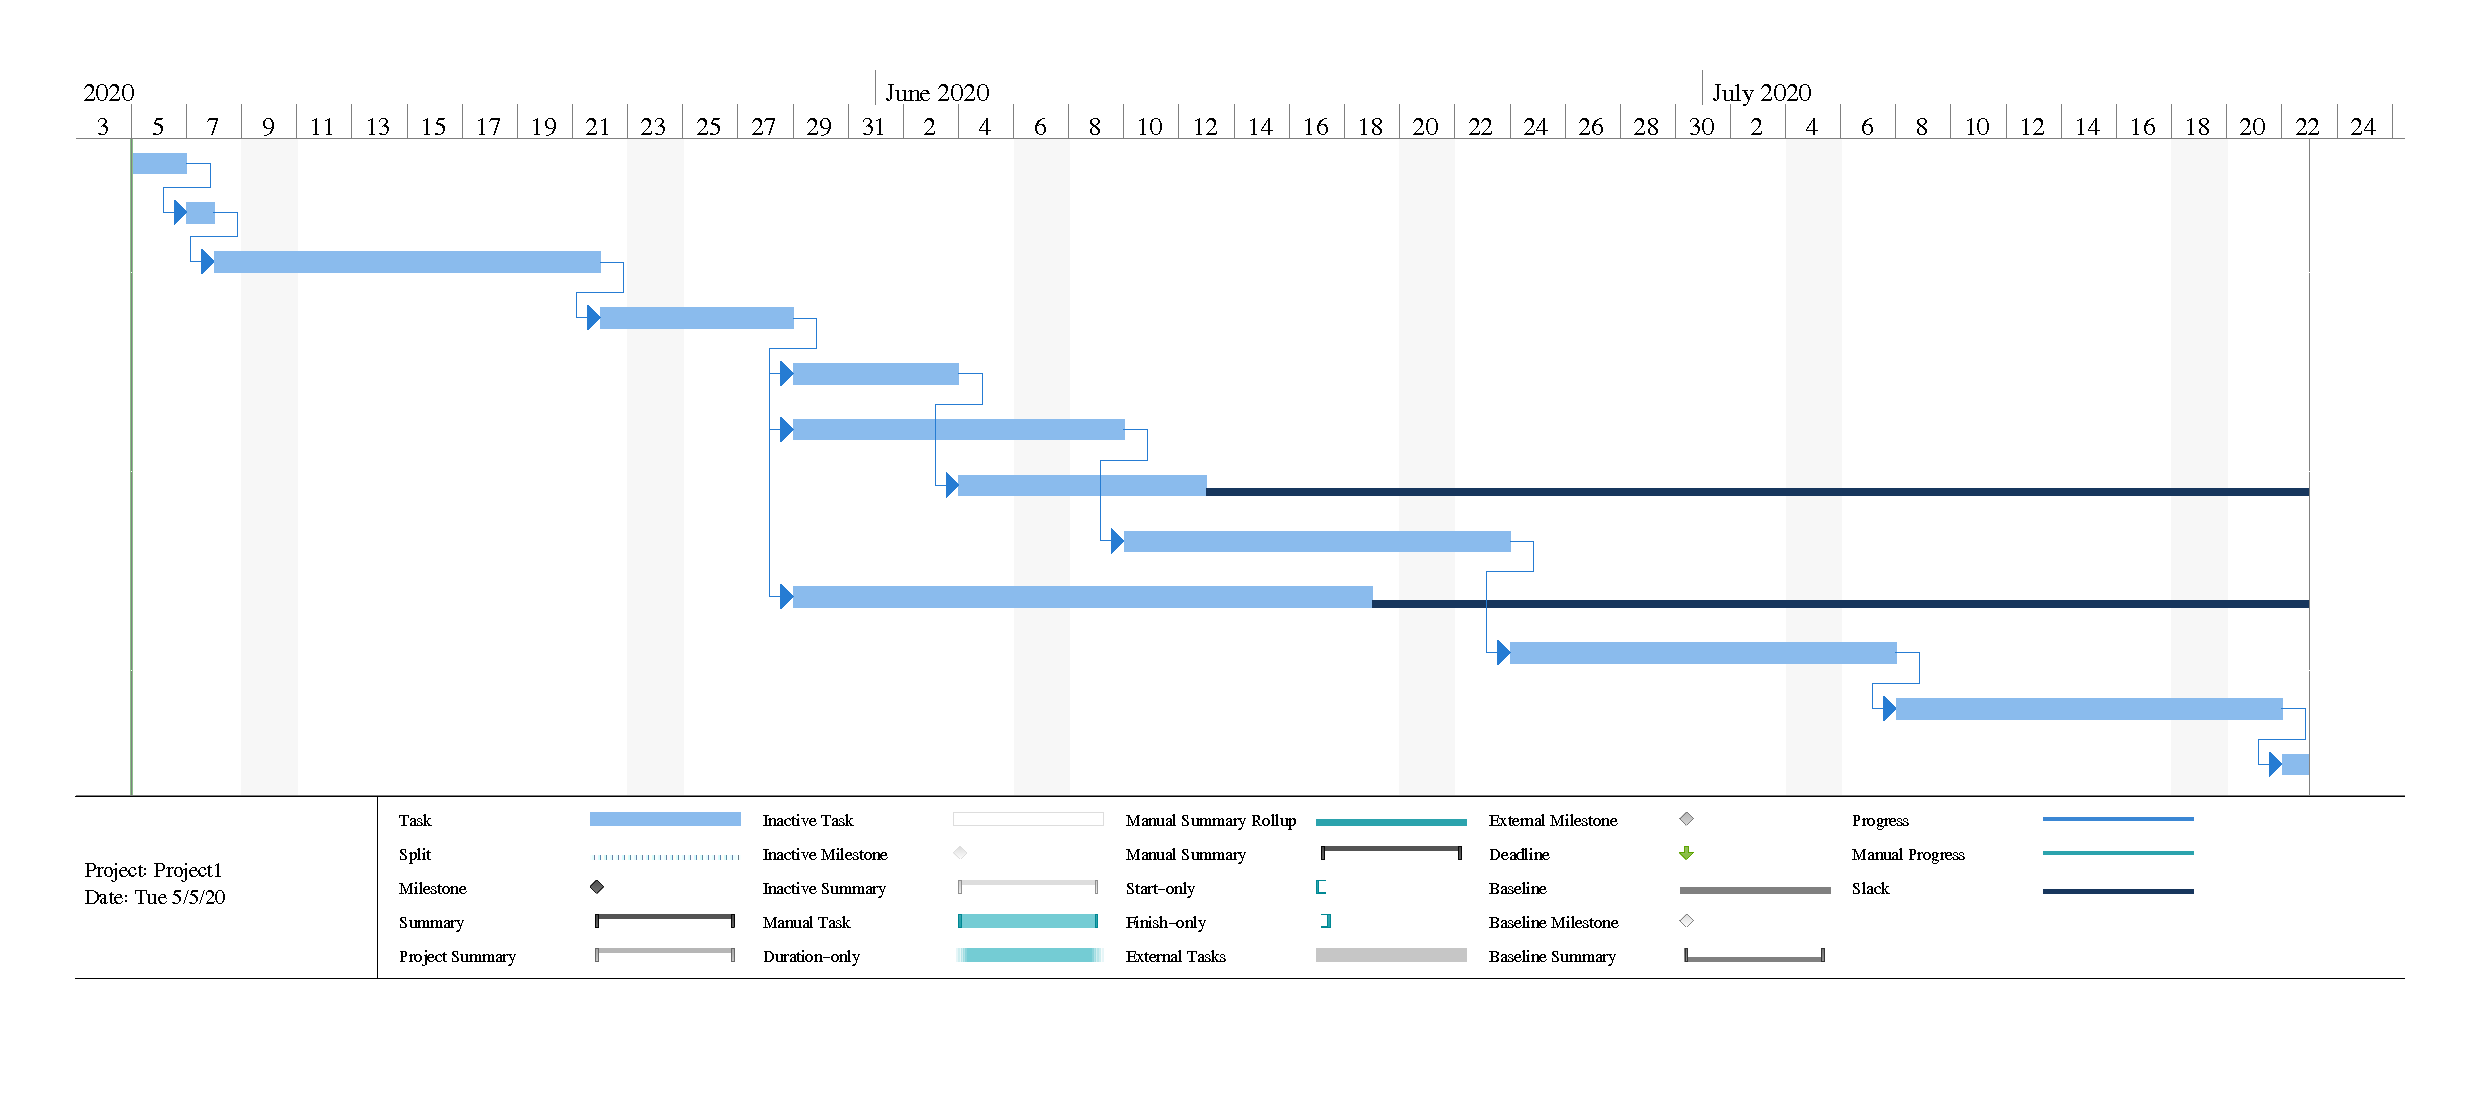
\includegraphics[width=\textwidth]{diagrams/gantchart.pdf}
				\caption{نمودار گانت}
				\label{subfig1:fig1:sec5:chap1}
			\end{subfigure}
		\end{flushleft}
	\end{figure}

	\pagebreak
	\section{
		نمودار
		BPMN}\label{sec7:chap1}
	نمودار 
	\lr{BPMN}
	استانداردی برای مدل‌سازی و نمایش فرایند‌های کسب‌و‌کار است. هدف اصلی در شکل گیری
	\lr{BPMN}،
	طراحی نمادهایی است که قابل‌درک برای تمامی کابران فرایند (از تحلیلگران فرایند کاری 
	\lr{(Business Analysts)}
	تا کاربران فنی 
	\lr{(Technical Developers)}
	و حتی کاربرانی که پایش و کنترل فرایند را بر عهده‌دارند) باشد.
	\begin{figure}[!h]
		\label{fig1:sec6:chap1}
		\begin{center}
			\begin{subfigure}[t]{\textwidth}
				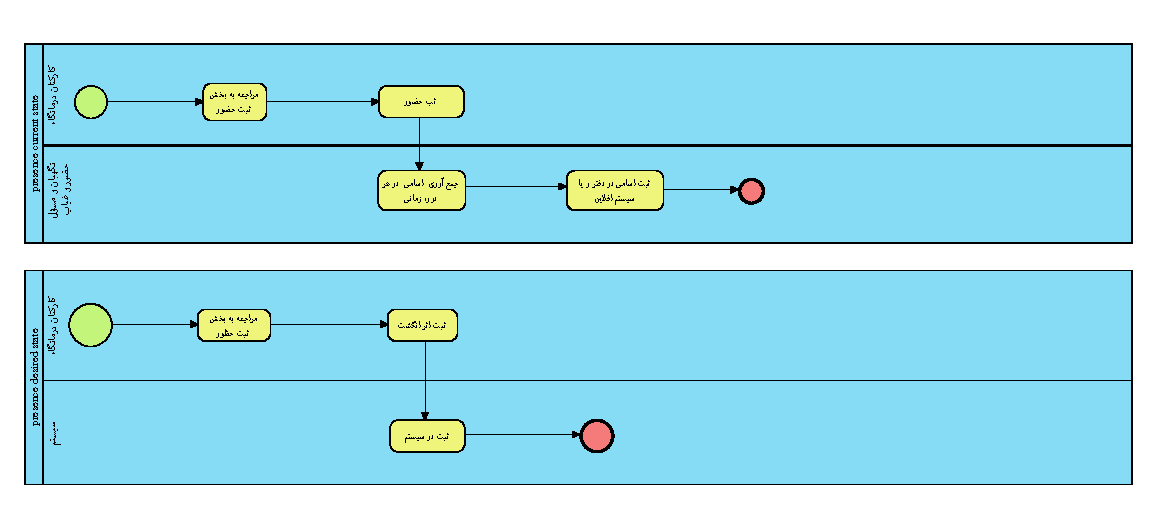
\includegraphics[width=\textwidth]{diagrams/employeePresence.pdf}
				\caption{حضور غیاب کارکنان (حالت موجود و مطلوب)}
				\label{subfig1:fig1:sec6:chap1}
			\end{subfigure}
			\begin{subfigure}[t]{\textwidth}
				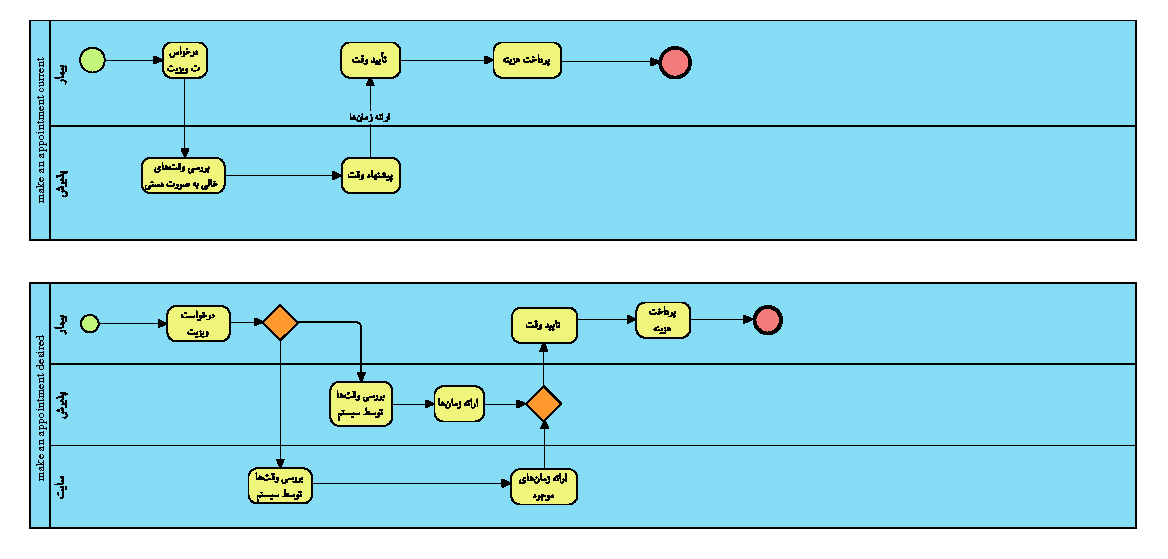
\includegraphics[width=\textwidth]{diagrams/makeAnAppointment.pdf}
				\caption{وقت گرفتن (حالت موجود و مطلوب)}
				\label{subfig2:fig1:sec6:chap1}
			\end{subfigure}
		\end{center}
	\end{figure}


	\pagebreak
	\begin{figure}[!h]
		\label{fig2:sec6:chap1}
		\begin{center}
			\begin{subfigure}[t]{\textwidth}
				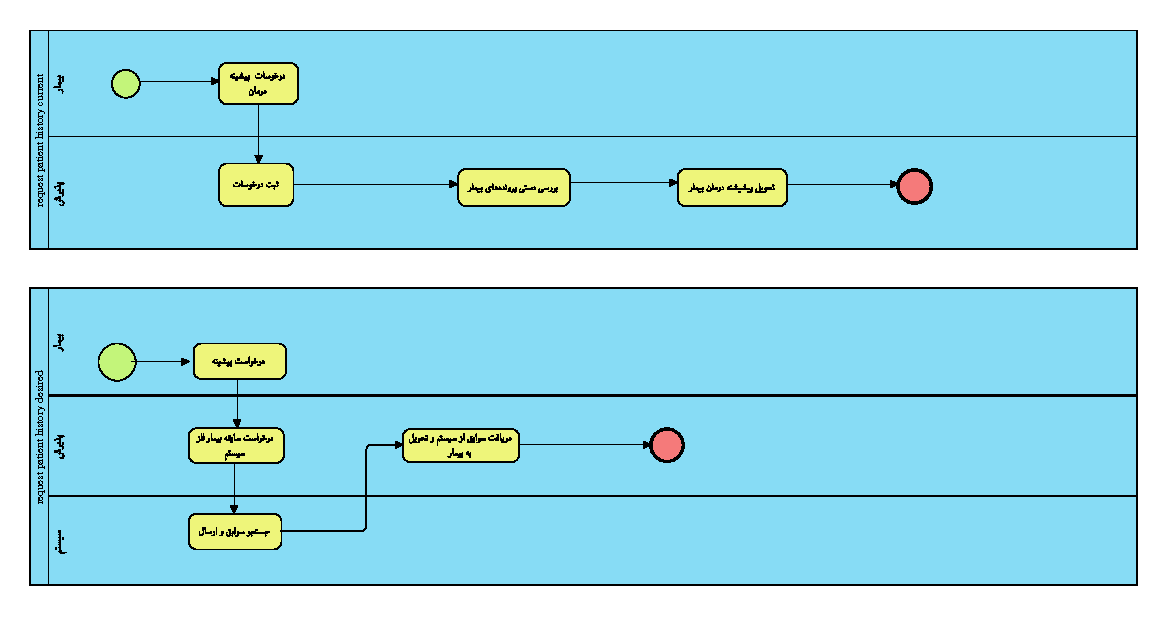
\includegraphics[width=\linewidth]{diagrams/requestPatientHistory.pdf}
				\caption{درخواست گزارش پیشینه درمان (حالت موجود و مطلوب)}
				\label{subfig3:fig1:sec6:chap1}
			\end{subfigure}	\\
			\begin{subfigure}[t]{\textwidth}
				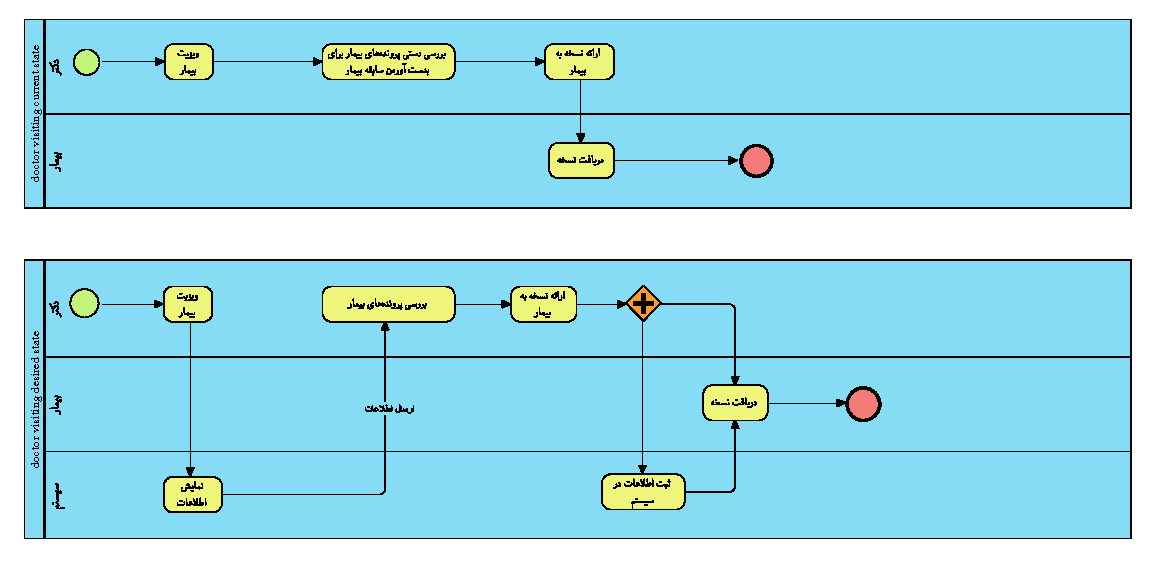
\includegraphics[width=\textwidth]{diagrams/visiting.pdf}
				\caption{ویزیت شدن بیمار(حالت موجود و مطلوب)}
				\label{subfig4:fig1:sec6:chap1}
			\end{subfigure}	
		\end{center}
	\end{figure}

	\pagebreak
	\chapter{
	مستندات پیاده سازی}
	\label{chp2}
	\noindent
	این فصل در مورد مستندات پیاده سازی، که شامل بخش‌های زیر است.
	\begin{itemize}
		\item 
		نمودار کاربرد، برای درک بهتر ارتباطات میان اجزاء سیستم.
		\item
		نمودار 
		\lr{ERD
		}، که یک ساختار کلی از پایگاه داده، شامل ارتباطات میان جدول‌ها و کلید‌های اصلی و خارجی را نشان می‌دهد.
		\item
		نمودار کلاس،‌ یک نمودار برای درک بهتر معماری و ساختار برنامه.
	\end{itemize}

	کد نرم‌افزار تحت مجوز 
	\lr{LGPLv3}
	در 
	\lr{Github}
	قرار دارد که می‌توانید از لینک زیر آن را مشاهده کنید. 
	
	\url{https://github.com/SMR76/clinic-manegement}
	\pagebreak
	\section{
		نمودار 
	\lr{UseCase}}\label{sec1:chap2}
	\vspace{-2cm}
	\begin{figure}[!h]
		\label{fig1:sec1:chap2}
		\begin{center}
			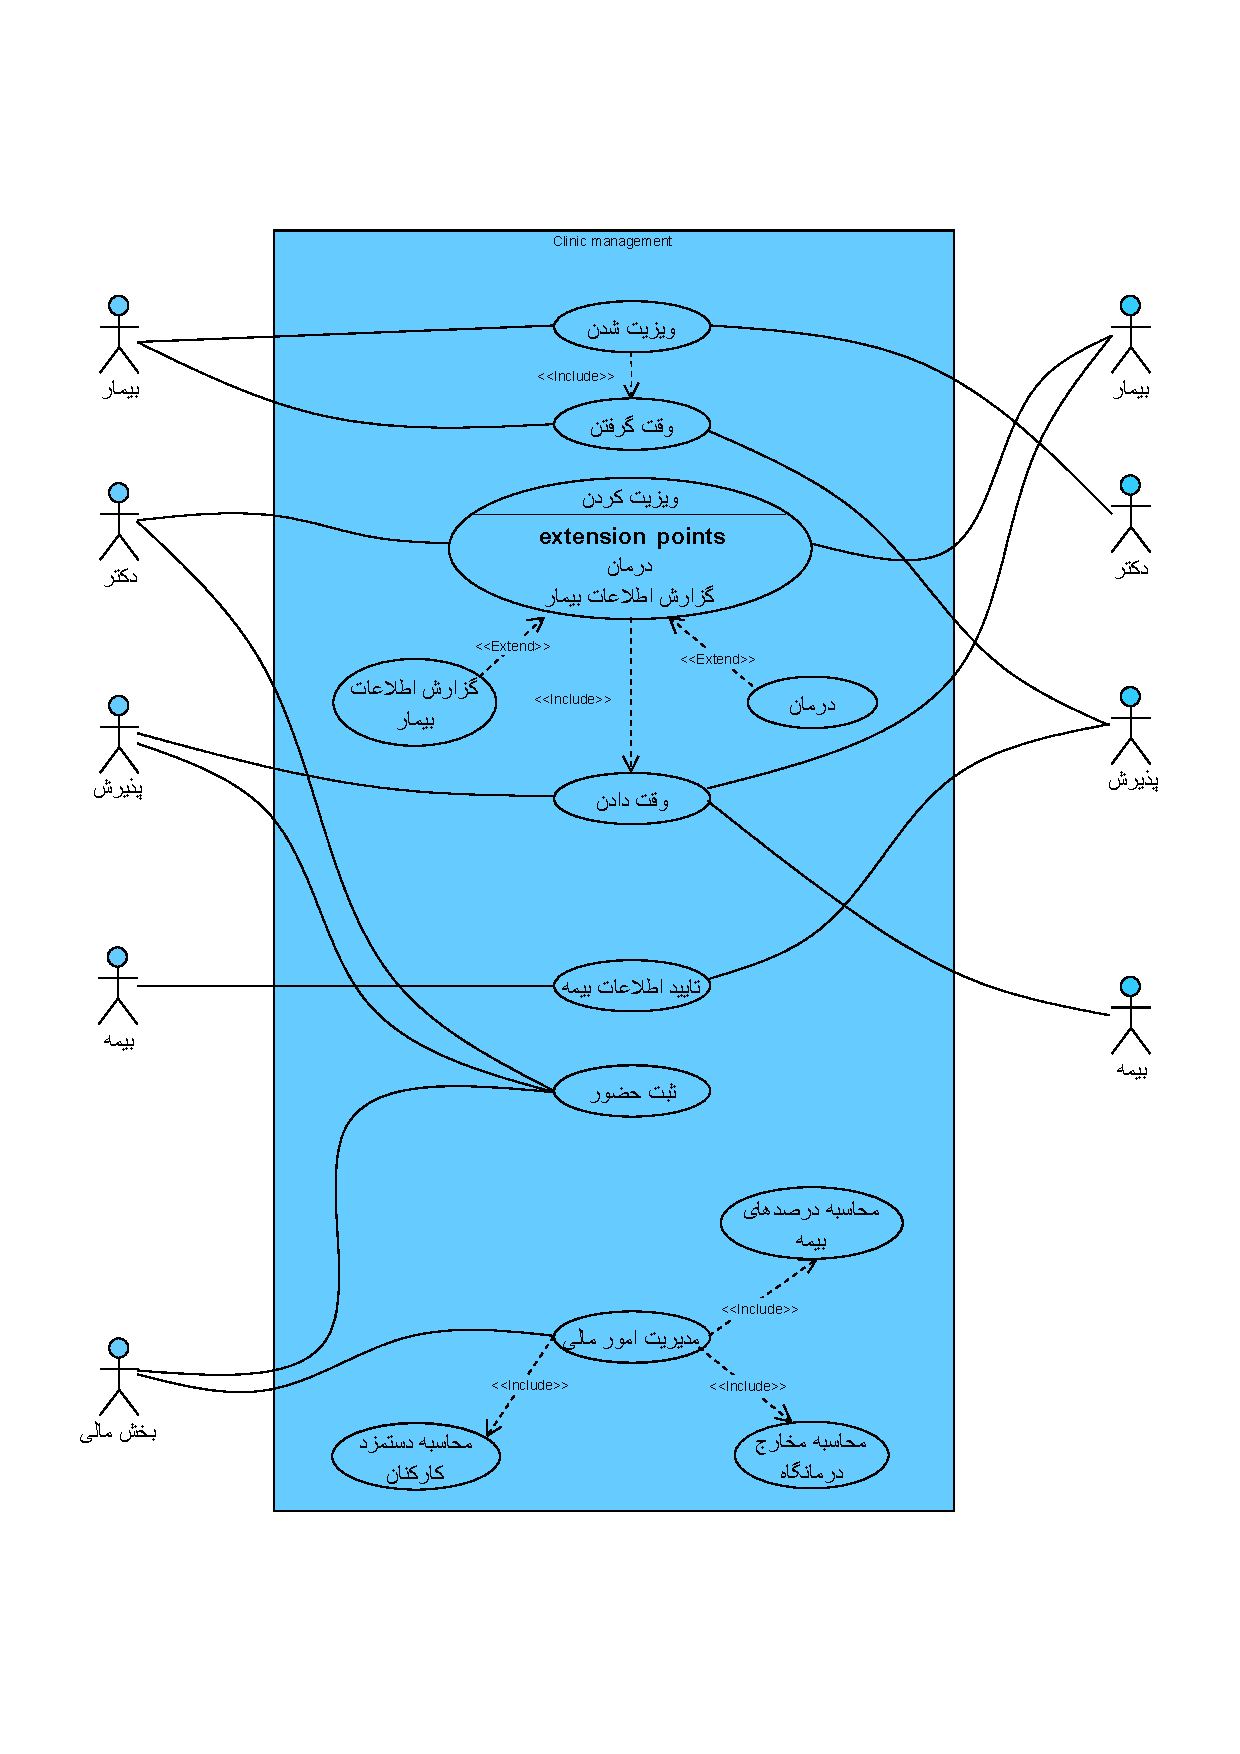
\includegraphics[width=0.7\textwidth]{diagrams/useCase.pdf}
			\caption{نمودار مورد کاربرد}
		\end{center}
	\end{figure}

	\pagebreak
	\section{
		نمودار 
		\lr{ERD}}\label{sec2:chap2}
	\begin{figure}[!h]
		\label{fig1:sec2:chap2}
		\begin{center}
			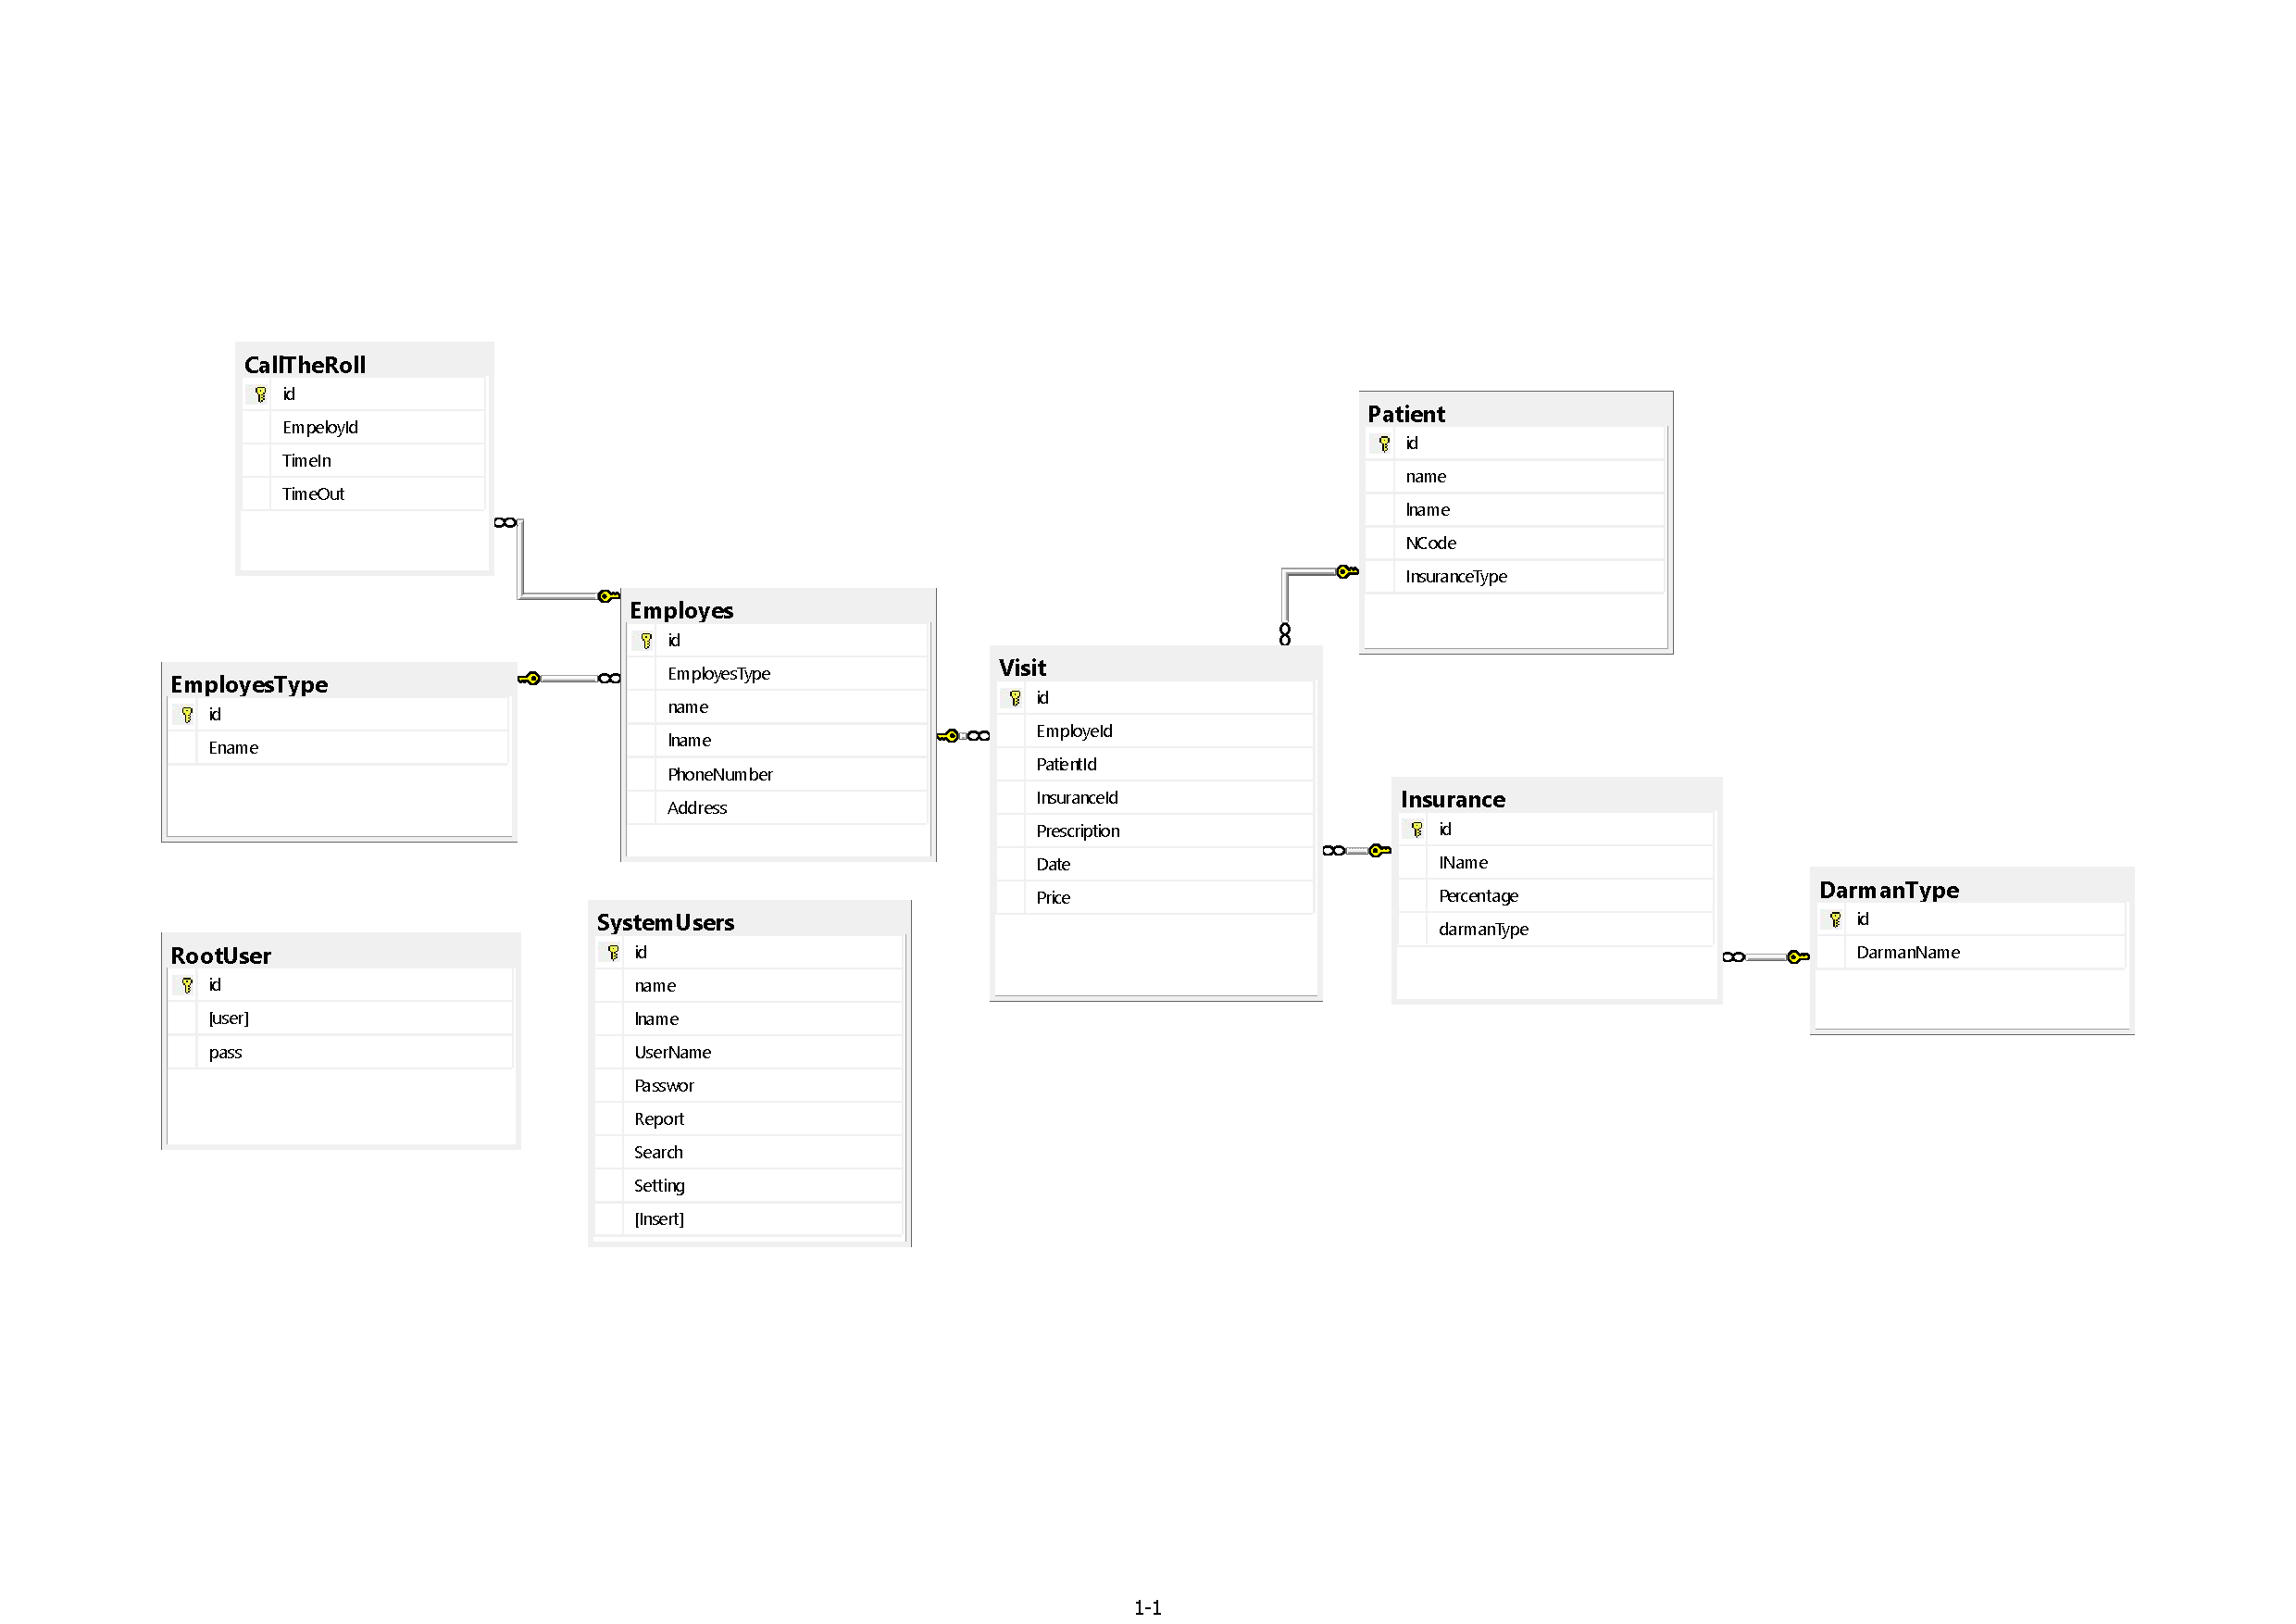
\includegraphics[width=0.8\textwidth]{diagrams/ERD.pdf}
			\caption{نمودار رابطه موجودیت‌ها}
		\end{center}
	\end{figure}


	\section{
		نمودار 
		\lr{Class}}\label{sec3:chap2}

	\begin{figure}[!h]
		\label{fig1:sec3:chap2}
		\begin{center}
			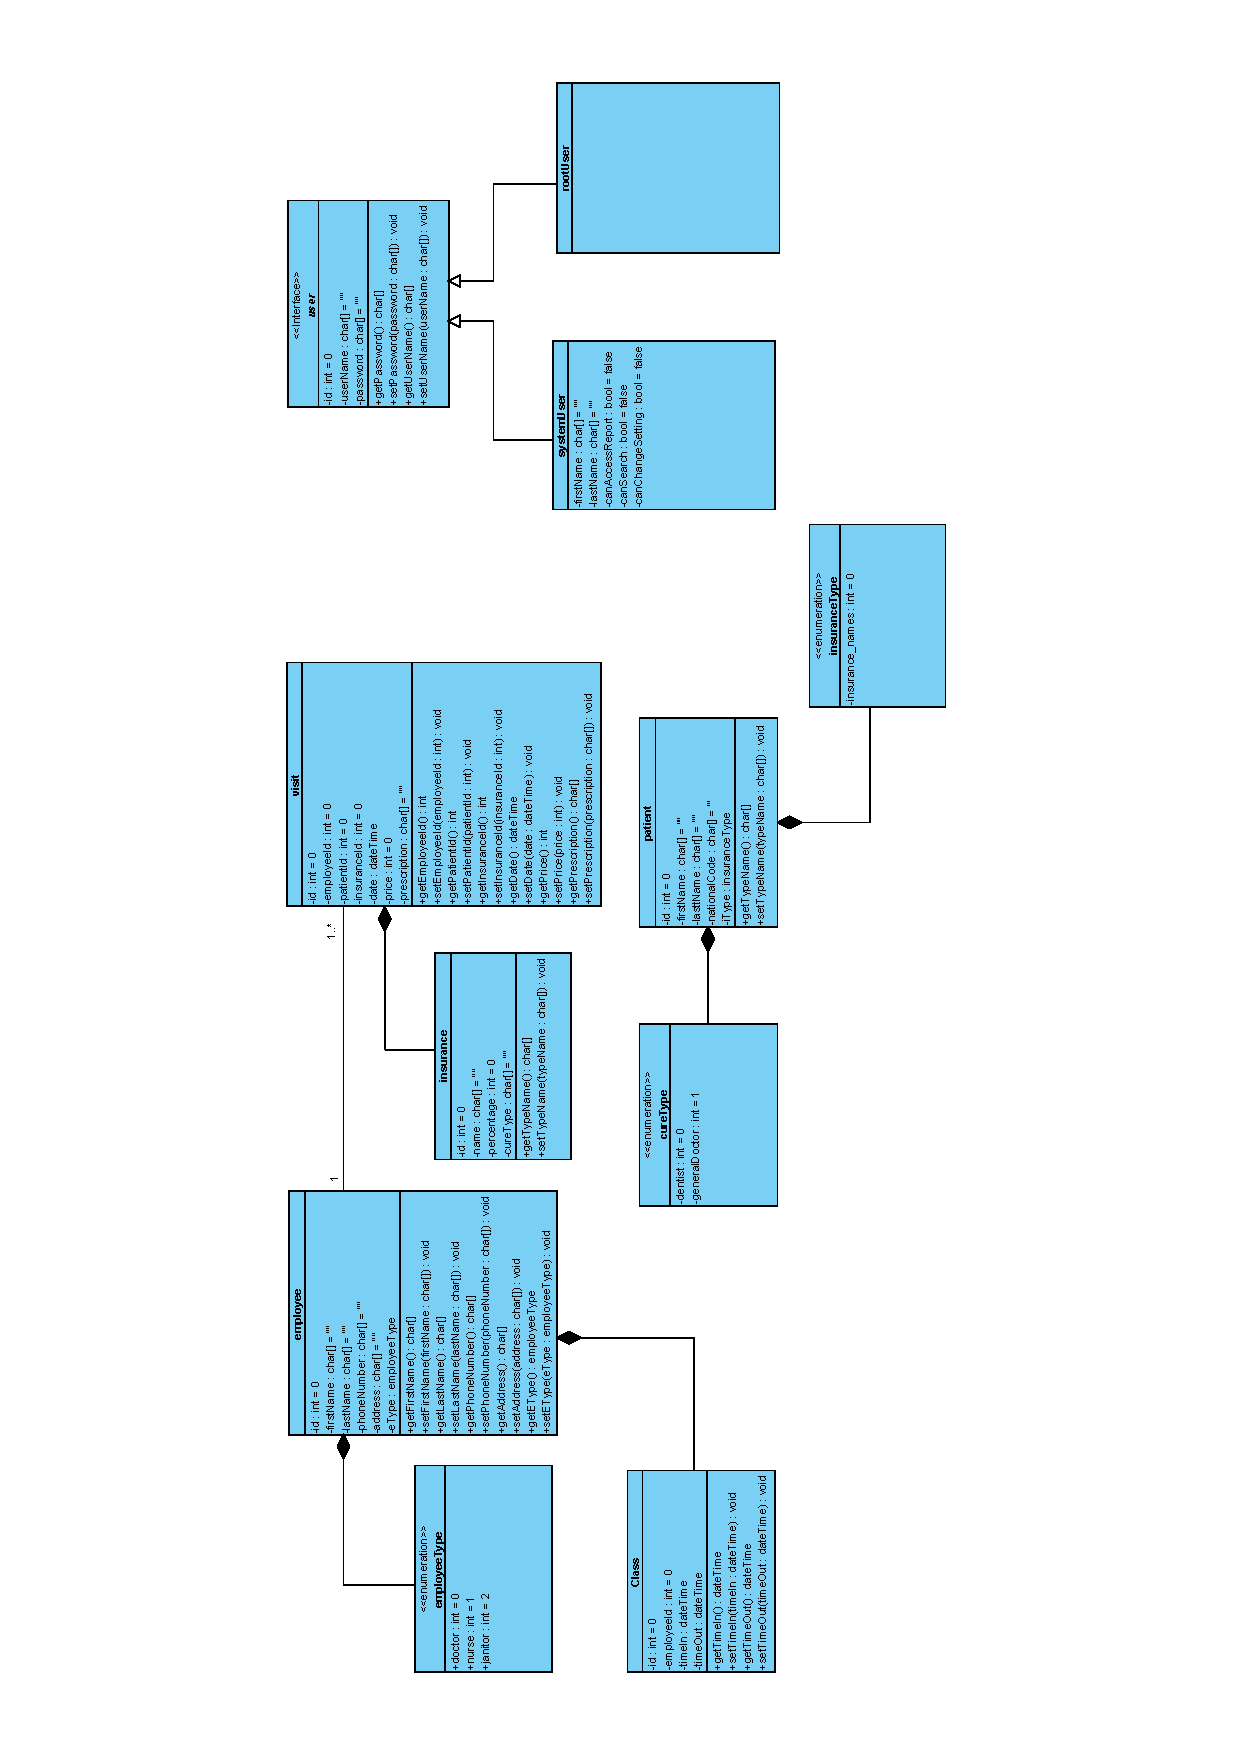
\includegraphics[width=0.8\textwidth]{diagrams/classDiagram.pdf}
			\caption{نمودار کلاس}
		\end{center}
	\end{figure}

	\chapter{
		رابط کاربری}
	\label{chp3}
	\section{
	رابط کاربری دسکتاپ (پیشنهادی)
	}\label{sec1:chap3}

	\begin{figure}[!h]
		\label{fig1:sec1:chap3}
		\begin{center}
			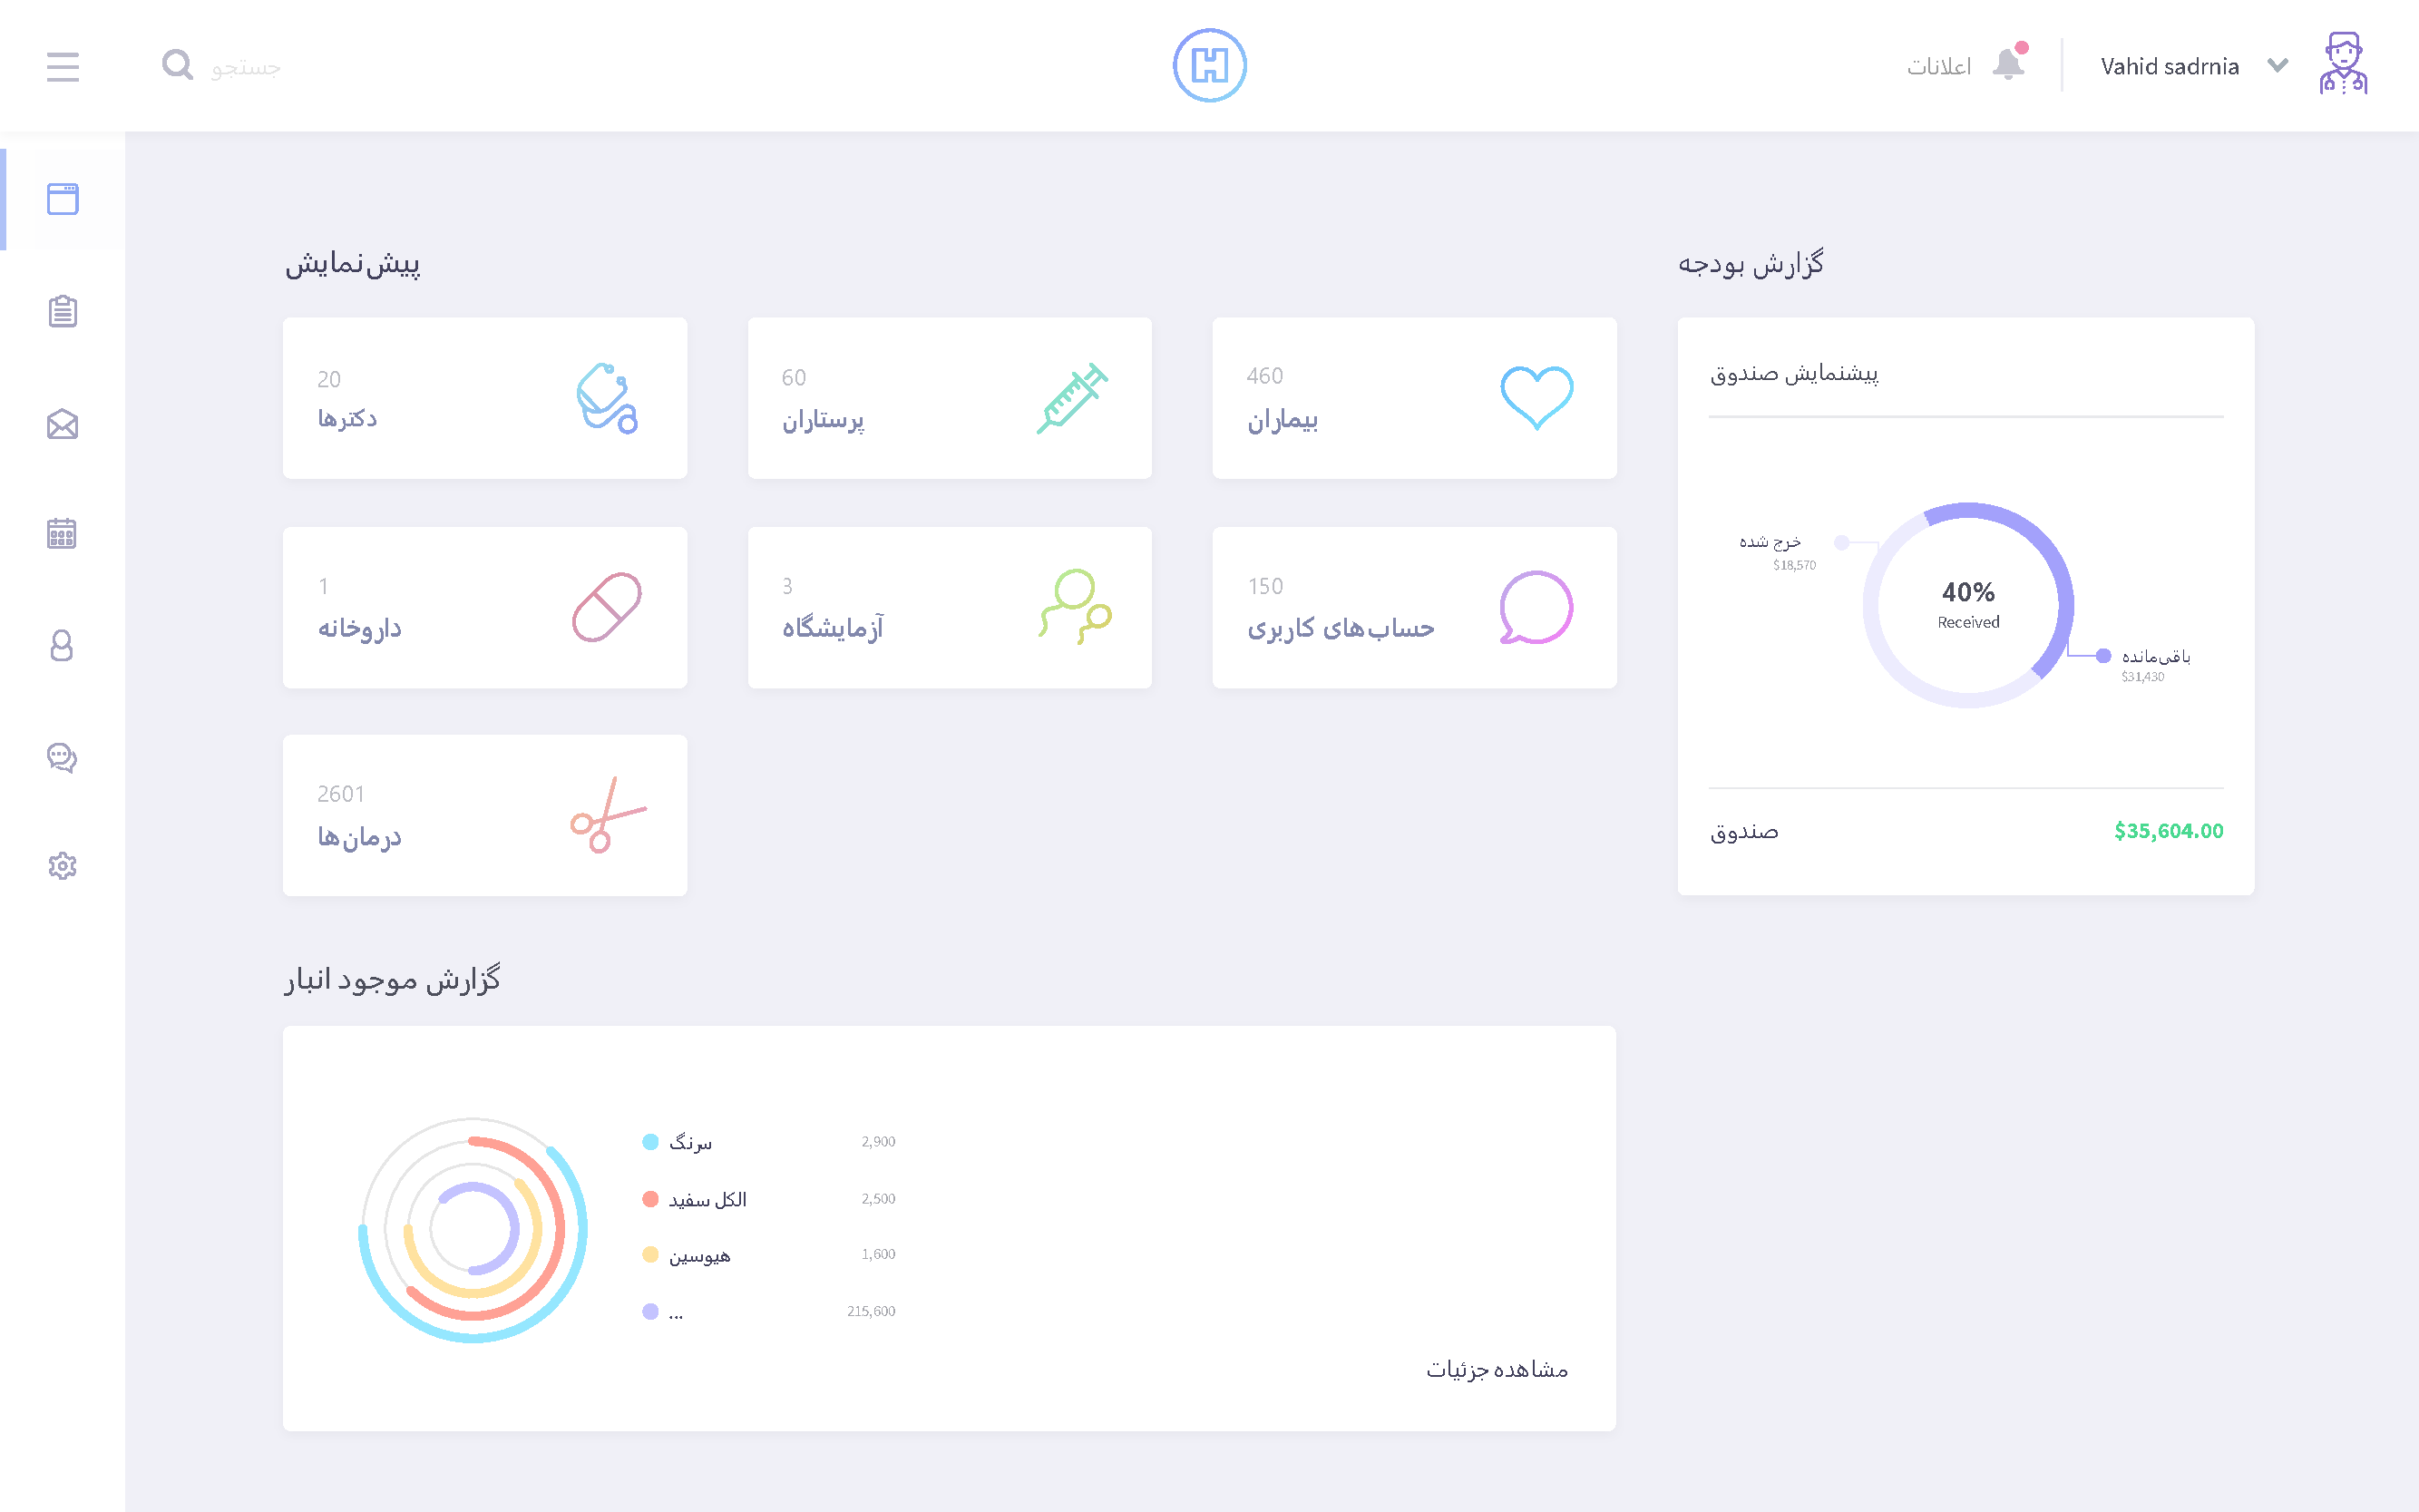
\includegraphics[width=0.8\textwidth]{UI/Desktop-UI.pdf}
			\caption{
			رابط کاربری طراحی شده برای نسخه دسکتاپ (هنوز اجرایی نشده)
			}
		\end{center}
	\end{figure}

	\section{
		رابط کاربری دسکتاپ (پیشنهادی)
	}\label{sec2:chap3}
	
	\begin{figure}[!h]
		\centering
		\begin{subfigure}[t]{0.3\linewidth}
			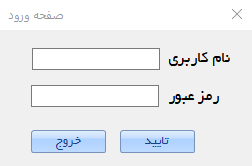
\includegraphics[width=0.9\textwidth]{UI/Desktop_UI_1.png}
		\end{subfigure}
		\begin{subfigure}[t]{0.3\linewidth}
			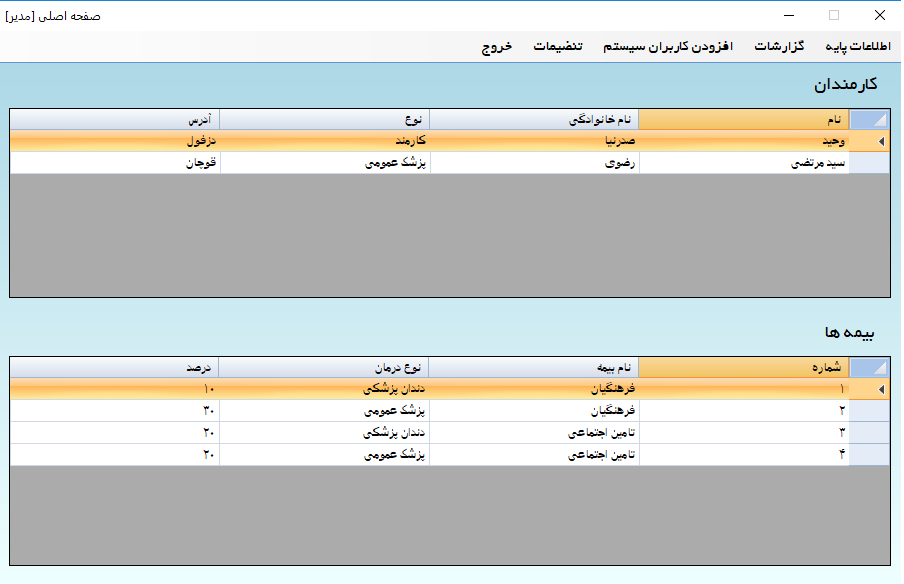
\includegraphics[width=0.9\textwidth]{UI/Desktop_UI_2.PNG}
		\end{subfigure}
		\begin{subfigure}[t]{0.3\linewidth}
			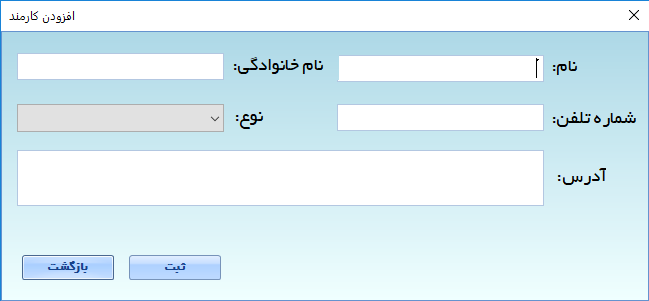
\includegraphics[width=0.9\textwidth]{UI/Desktop_UI_3.PNG}
		\end{subfigure}
		\par\bigskip
		\vspace*{3mm}		
		\begin{subfigure}[t]{0.3\linewidth}
			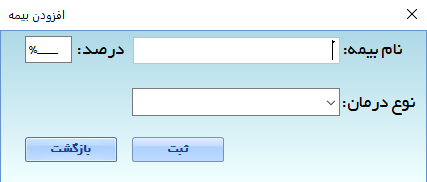
\includegraphics[width=0.9\textwidth]{UI/Desktop_UI_4.png}
		\end{subfigure}
		\begin{subfigure}[t]{0.3\linewidth}
			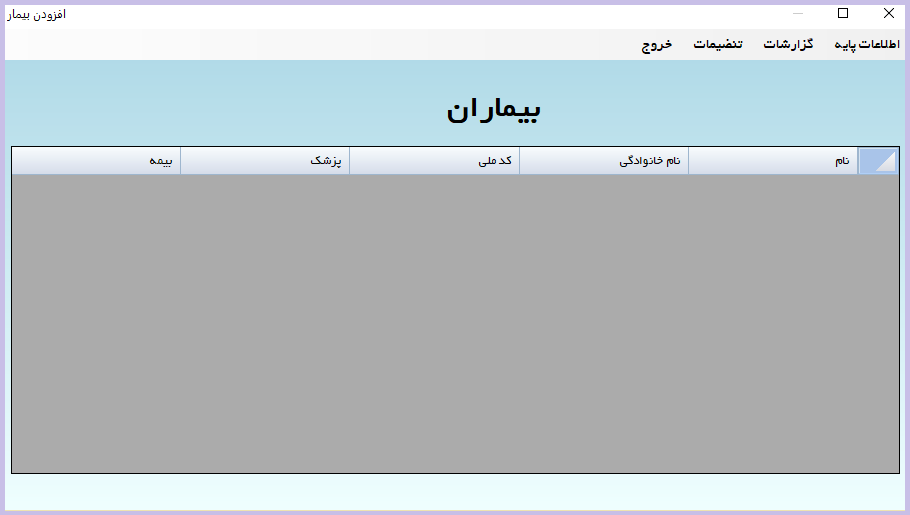
\includegraphics[width=0.9\textwidth]{UI/Desktop_UI_5.PNG}
		\end{subfigure}
		\begin{subfigure}[t]{0.3\linewidth}
			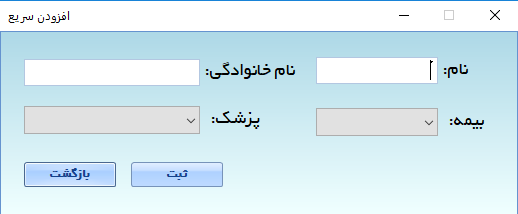
\includegraphics[width=0.9\textwidth]{UI/Desktop_UI_6.PNG}
		\end{subfigure}
		\par\bigskip
		\vspace*{3mm}		
		\begin{subfigure}[t]{0.6\linewidth}
			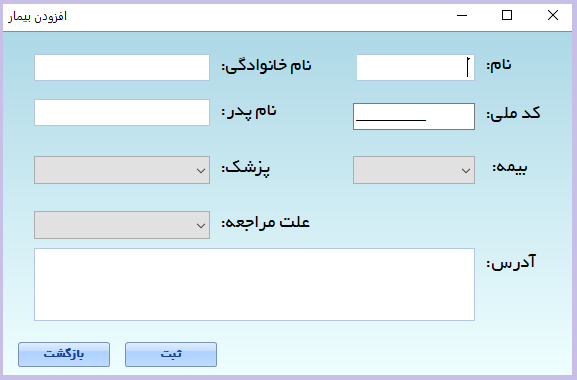
\includegraphics[width=0.9\textwidth]{UI/Desktop_UI_7.PNG}
		\end{subfigure}
		\label{fig1:sec2:chap3}
		\caption{
			رابط کاربری کنونی برای دسکتاپ
		}
	\end{figure}
	
\end{document}